% Options for packages loaded elsewhere
\PassOptionsToPackage{unicode}{hyperref}
\PassOptionsToPackage{hyphens}{url}
%
\documentclass[
]{article}
\usepackage{amsmath,amssymb}
\usepackage{iftex}
\ifPDFTeX
  \usepackage[T1]{fontenc}
  \usepackage[utf8]{inputenc}
  \usepackage{textcomp} % provide euro and other symbols
\else % if luatex or xetex
  \usepackage{unicode-math} % this also loads fontspec
  \defaultfontfeatures{Scale=MatchLowercase}
  \defaultfontfeatures[\rmfamily]{Ligatures=TeX,Scale=1}
\fi
\usepackage{lmodern}
\ifPDFTeX\else
  % xetex/luatex font selection
\fi
% Use upquote if available, for straight quotes in verbatim environments
\IfFileExists{upquote.sty}{\usepackage{upquote}}{}
\IfFileExists{microtype.sty}{% use microtype if available
  \usepackage[]{microtype}
  \UseMicrotypeSet[protrusion]{basicmath} % disable protrusion for tt fonts
}{}
\makeatletter
\@ifundefined{KOMAClassName}{% if non-KOMA class
  \IfFileExists{parskip.sty}{%
    \usepackage{parskip}
  }{% else
    \setlength{\parindent}{0pt}
    \setlength{\parskip}{6pt plus 2pt minus 1pt}}
}{% if KOMA class
  \KOMAoptions{parskip=half}}
\makeatother
\usepackage{xcolor}
\usepackage[margin=1in]{geometry}
\usepackage{graphicx}
\makeatletter
\def\maxwidth{\ifdim\Gin@nat@width>\linewidth\linewidth\else\Gin@nat@width\fi}
\def\maxheight{\ifdim\Gin@nat@height>\textheight\textheight\else\Gin@nat@height\fi}
\makeatother
% Scale images if necessary, so that they will not overflow the page
% margins by default, and it is still possible to overwrite the defaults
% using explicit options in \includegraphics[width, height, ...]{}
\setkeys{Gin}{width=\maxwidth,height=\maxheight,keepaspectratio}
% Set default figure placement to htbp
\makeatletter
\def\fps@figure{htbp}
\makeatother
\setlength{\emergencystretch}{3em} % prevent overfull lines
\providecommand{\tightlist}{%
  \setlength{\itemsep}{0pt}\setlength{\parskip}{0pt}}
\setcounter{secnumdepth}{-\maxdimen} % remove section numbering
\usepackage{titlesec}
\titleformat*{\section}{\normalfont\Large\bfseries\flushleft}
\titleformat*{\subsection}{\normalfont\large\bfseries\flushleft}
\titleformat*{\subsubsection}{\normalfont\normalsize\bfseries\flushleft}
\usepackage{amsmath}
\newcommand*{\defeq}{\mathrel{\vcenter{\baselineskip0.5ex \lineskiplimit0pt \hbox{\scriptsize.}\hbox{\scriptsize.}}}=}
\newcommand*{\eqdef}{=\mathrel{\vcenter{\baselineskip0.5ex \lineskiplimit0pt \hbox{\scriptsize.}\hbox{\scriptsize.}}}}
\ifLuaTeX
  \usepackage{selnolig}  % disable illegal ligatures
\fi
\usepackage{bookmark}
\IfFileExists{xurl.sty}{\usepackage{xurl}}{} % add URL line breaks if available
\urlstyle{same}
\hypersetup{
  pdftitle={Statistical Learning (5454) - Assignment 3},
  pdfauthor={Matthias Hochholzer, Lukas Pirnbacher, Anne Valder},
  hidelinks,
  pdfcreator={LaTeX via pandoc}}

\title{Statistical Learning (5454) - Assignment 3}
\author{Matthias Hochholzer, Lukas Pirnbacher, Anne Valder}
\date{Due: 2024-05-20}

\begin{document}
\maketitle

\section{Exercise 1}\label{exercise-1}

We load the data set \texttt{Carseats} from package \textbf{ISLR2}. It
is a simulated data set containing sales of child car seats at 400
different stores. We then randomly select 280 observations as training
data and use the remaining ones as test data (70:30 split).

Next, we fit a regression tree to the training set. We set the
complexity parameter to \(cp = 10^{-4}\) in order to initially grow a
rather large tree, which we intend to prune later on.

\begin{verbatim}
## 
## Regression tree:
## rpart(formula = Sales ~ ., data = train, method = "anova", control = list(cp = 1e-04))
## 
## Variables actually used in tree construction:
## [1] Advertising Age         CompPrice   Price      
## [5] ShelveLoc  
## 
## Root node error: 2227/280 = 8
## 
## n= 280 
## 
##        CP nsplit rel error xerror  xstd
## 1  0.2546      0      1.00   1.01 0.085
## 2  0.0922      1      0.75   0.76 0.059
## 3  0.0709      2      0.65   0.74 0.058
## 4  0.0432      3      0.58   0.63 0.048
## 5  0.0360      4      0.54   0.63 0.051
## 6  0.0323      5      0.50   0.63 0.053
## 7  0.0243      7      0.44   0.59 0.049
## 8  0.0175      8      0.41   0.59 0.048
## 9  0.0159      9      0.40   0.61 0.053
## 10 0.0156     10      0.38   0.62 0.053
## 11 0.0141     11      0.37   0.61 0.053
## 12 0.0135     12      0.35   0.60 0.053
## 13 0.0127     14      0.32   0.60 0.052
## 14 0.0105     15      0.31   0.58 0.052
## 15 0.0092     16      0.30   0.59 0.052
## 16 0.0089     17      0.29   0.58 0.052
## 17 0.0078     18      0.28   0.58 0.051
## 18 0.0069     20      0.27   0.57 0.051
## 19 0.0068     21      0.26   0.57 0.052
## 20 0.0053     22      0.25   0.56 0.051
## 21 0.0049     23      0.25   0.55 0.051
## 22 0.0037     24      0.24   0.55 0.051
## 23 0.0001     25      0.24   0.55 0.050
\end{verbatim}

A plot of the complexity parameter table and the plot of the tree can be
seen below.

\begin{center}\includegraphics{A3_files/figure-latex/unnamed-chunk-5-1} \end{center}

\includegraphics{A3_files/figure-latex/unnamed-chunk-6-1.pdf}

The fitted tree has 26 terminal nodes (25 splits). Overall, 5 of the 10
available predictors are used in the construction of the tree (shelf
location, price, price of competitor, average age of the local
population, advertising budget). Since the tree is rather long we do
further interpretations with the pruned tree.

Given the loose stopping criterion we chose, we are in principle facing
the risk of overiftting. In order to solve this problem, we prune the
tree later on. However, as the cross-validated errors (\texttt{xerror})
are not increasing for smaller values of \texttt{cp}, we believe that
overfitting may not be a problem. For now, we calculate the test MSE for
the full tree, which is given by

\begin{verbatim}
## [1] 3.519
\end{verbatim}

We now use 10-fold cross-validation (which is the default in
\texttt{rpart()}) in order to determine the optimal level of tree
complexity. We do so by applying the 1-SE rule, i.e.~we choose the
largest complexity parameter such that the corresponding cross-validated
error is smaller than the minimum error plus one standard deviation.

\begin{verbatim}
## 
## Regression tree:
## rpart(formula = Sales ~ ., data = train, method = "anova", control = list(cp = 1e-04))
## 
## Variables actually used in tree construction:
## [1] CompPrice Price     ShelveLoc
## 
## Root node error: 2227/280 = 8
## 
## n= 280 
## 
##      CP nsplit rel error xerror  xstd
## 1 0.255      0      1.00   1.01 0.085
## 2 0.092      1      0.75   0.76 0.059
## 3 0.071      2      0.65   0.74 0.058
## 4 0.043      3      0.58   0.63 0.048
## 5 0.036      4      0.54   0.63 0.051
## 6 0.032      5      0.50   0.63 0.053
## 7 0.024      7      0.44   0.59 0.049
\end{verbatim}

\includegraphics{A3_files/figure-latex/unnamed-chunk-8-1.pdf}
\includegraphics{A3_files/figure-latex/unnamed-chunk-8-2.pdf}

The pruned tree has 8 terminal nodes (7 splits). In contrast to the full
tree, the advertising budget as well as the average age of the local
population are no longer used to construct the tree. The first split is
made according to the quality of the shelving location for the car
seats. It splits into \textit{Bad \& Medium} and \textit{Good}. The
second split is based on the car seat price for a \textit{Bad \& Medium}
shelving location. The third split distinguishes between \textit{Bad}
and \textit{Medium} shelving location for products with higher prices.
For the medium shelving location there is another split based on the
price of the competitor. For low-price products with
\textit{Bad \& Medium} location there are two more splits based on the
competitor's and the own price. Finally, for products with \textit{Good}
shelving location, a split is made based upon the price. Looking at the
boxplots at each terminal node, it seems that even the last split was
still important.

Overall, the pruned tree displays quite intuitive patterns: Sales
increase with the quality of the shelving location, increase for higher
prices of the competitors and decrease as the price of the car seats
increases. It is interesting, though, that the price of competitors is a
relevant explanatory factor only for car seats in bad or medium shelving
locations.

The test MSE with pruning is

\begin{verbatim}
## [1] 4.353
\end{verbatim}

and therefore higher than for the initial tree. Hence, pruning the tree
does not improve the test MSE, which indicates that overfitting was
actually not too much of a problem. However, while pruning has not
improved the predictive performance of the tree, it has significantly
simplified the interpretation.

\newpage

\section{Exercise 2}\label{exercise-2}

We draw 100 observations from four independent variables
\(X_1,\ldots,X_4\), where

\begin{itemize}
  \item $X_1$ follows a standard uniform distribution,
  \item $X_2$ follows a standard normal distribution,
  \item $X_3$ follows a Bernoulli distribution with success probability $\pi = 0.5$,
  \item $X_4$ follows a Bernoulli distribution with success probability $\pi = 0.1$.
\end{itemize}

We now repeat the following 1000 times:

\begin{itemize}
  \item Draw a dependent variable $y$ from a standard normal distribution, which is independent of the four independent variables.
  \item Fit a tree stump, i.e. a tree which contains only one split.
  \item Determine which variable was used for splitting.
\end{itemize}

Below is the table of relative frequencies, displaying how often each of
the variables was selected for splitting. We also provide a barplot to
visualize the findings.

\begin{verbatim}
## 
##    X1    X2    X3    X4 
## 0.460 0.471 0.037 0.032
\end{verbatim}

\includegraphics{A3_files/figure-latex/unnamed-chunk-11-1.pdf}

The probability of including a particular independent variable is not
the same. \(X_2\) has the highest probability, closely followed by
\(X_1\). The inclusion probabilities for \(X_3\) and \(X_4\) are much
lower. Hence, while all predictors are independent of \(y\), the two
continuous variables (\(X_1, X_2\)) are much more likely to be selected
as splitting variable. This should not come as a surprise, as a
continuous split variable allows for more flexibility in partitioning
the \(X\)-space. By choosing different split points, one can define a
wide variety of different pairs of half-planes. For a binary split
variable, in contrast, there is only a single possible partition, with
all observations where the split variable is equal to 1 being part of
one region and the remaining observations being part of the other
region. Thus, the probability of finding a partition of \(X\)-space such
that the sum of squared residuals is (by chance) small, is much higher
for continuous split variables.

\section{Exercise 3}\label{exercise-3}

We assume the following data generating process \[ Y = X + \epsilon, \]
with \(X \sim N(0,1)\) and \(\epsilon \sim N(0,1)\) independent. In
addition, 20 covariates \(Z_1,\ldots,Z_{20}\) are given with
\[Z_i \sim \sqrt{0.9}X + \epsilon_{Z_i},\] where
\(\epsilon_{Z_i} \sim N(0, 0.1)\).

We draw training data with 30 observations and test data with 10,000
observations from the data generating process, including the additional
covariates \(\mathbf{Z}\).

We then create 100 bootstrap samples of size 30 from the training data
by drawing with replacement.

To each bootstrap sample we fit:

\begin{enumerate}
\item a regression tree,
\item the null model with predicted value equal to the observed empirical mean of $Y$,
\item a linear model including linear effects for $X$ and all $Z$ variables and
\item a linear model potentially including linear effects for $X$ and all $Z$ variables, but using model selection
with the AIC to select a suitable model starting from the null model.
\end{enumerate}

We determine the predicted values on the test data for the bagged model
estimator by calculating the average predictions over the 100 trees
fitted to the bootstrap samples, the 100 null models, the 100 linear
models including all linear effects and the 100 linear models based on
model selection.

Finally, we determine the mean squared error (MSE) of the four bagged
model estimators on the test sample of size 10,000.

\begin{verbatim}
##   Model   MSE
## 1  Tree 1.211
## 2  Null 2.036
## 3    LM 4.436
## 4   AIC 1.765
\end{verbatim}

The lowest MSE is achieved by the regression tree, followed by the model
selected by AIC and the null model. The highest MSE is obtained in case
of the linear model including \(X\) and all \(Z\) variables, which
ultimately suffers from high multicollinearity.

\newpage

\section{Exercise 4}\label{exercise-4}

We load the dataset \texttt{icu} in package \textbf{aplore3}, which
contains information on patients who were admitted to an adult intensive
care unit (ICU). We drop the variable \texttt{id}, which is just an ID
number of the patients, and use the variable \texttt{sta} as dependent
variable in order to develop a predictive model of the patients'
survival.

We first fit a random forest using the default settings of
\texttt{randomForest()} for the number of bootstrap iterations
(\(ntree = 500\)) and the number of candidate variables at each split
(\(m = \sqrt{p}\), where \(p\) is the number of predictors).

\begin{verbatim}
## 
## Call:
##  randomForest(formula = sta ~ ., data = icu, importance = TRUE) 
##                Type of random forest: classification
##                      Number of trees: 500
## No. of variables tried at each split: 4
## 
##         OOB estimate of  error rate: 16%
## Confusion matrix:
##       Lived Died class.error
## Lived   153    7     0.04375
## Died     25   15     0.62500
\end{verbatim}

We now want to evaluate whether the default value of 500 bootstrap
iterations is sufficiently large. In order to do so, we look at the
evolution of the OOB error rate for increasing number of trees.
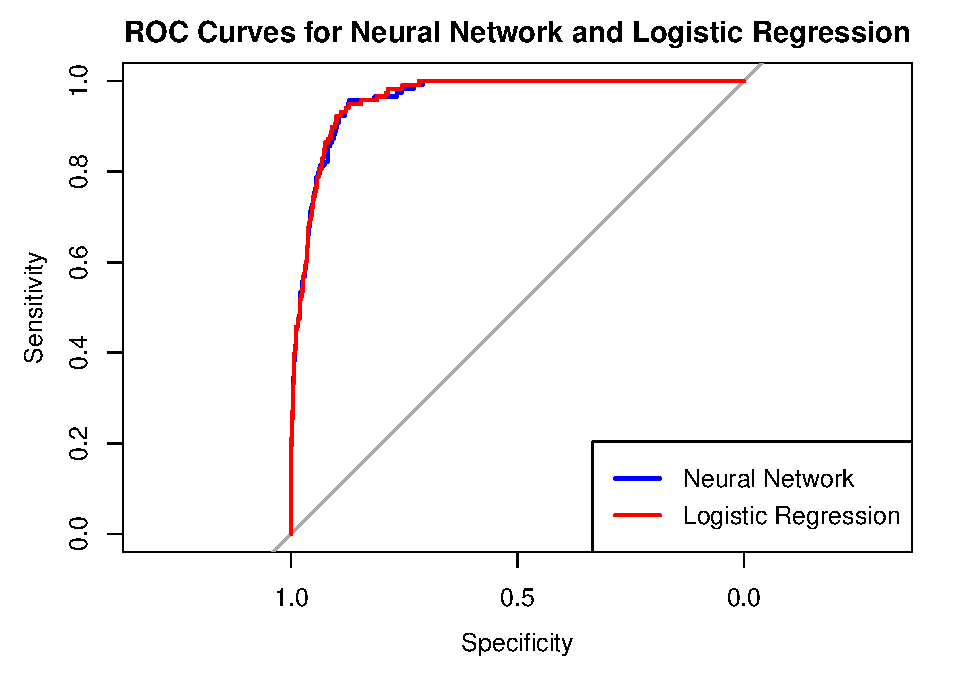
\includegraphics{A3_files/figure-latex/unnamed-chunk-19-1.pdf} The plot
shows that the error rates stabilize rather quickly and that 150 to 200
bootstrap iterations seem to be enough. However, since computational
costs are limited in this exercise we continue our analysis with
\(ntree = 500\).

Next, we want to tune the hyperparameter \(m\) and assess its influence
on the OOB error. Since the dataset is rather small, we consider all
possible values \(m = 1,\ldots 19\).

\begin{verbatim}
##  m = 1  m = 2  m = 3  m = 4  m = 5  m = 6  m = 7  m = 8 
##  0.200  0.165  0.170  0.155  0.150  0.165  0.170  0.160 
##  m = 9 m = 10 m = 11 m = 12 m = 13 m = 14 m = 15 m = 16 
##  0.165  0.170  0.170  0.165  0.170  0.170  0.165  0.160 
## m = 17 m = 18 m = 19 
##  0.165  0.165  0.180
\end{verbatim}

We find that the OOB error rate is quite insensitive to the choice of
\(m\) and that even a choice of \(m=1\) does not drastically increase
the OOB error. The OOB error rate is minimized for \(m=5\) and we choose
this value for the final task of this exercise, where we want to inspect
the variable importance measures.

\includegraphics{A3_files/figure-latex/unnamed-chunk-21-1.pdf}

By far the most important variable according to mean decrease accuracy
(MDA) is the level of consciousness at ICU admission (\texttt{loc}),
followed by systolic blood pressure, type of admission (elective or
emergency), age and the type of service (medical or surgery). Based on
mean decrease Gini (MDG) as importance measure, four explanatory
variables stand out: Systolic blood pressure is the most important
predictor, followed by age, the level of consciousness and the heart
rate at ICU admission.

Looking at the \texttt{class} of the five most important variables
according to each measure, we find that the MDG favors numeric
predictors:

\begin{verbatim}
## [1] "Top 5 - MDA:"
\end{verbatim}

\begin{verbatim}
##       loc       sys      type       age       ser 
##  "factor" "integer"  "factor" "integer"  "factor"
\end{verbatim}

\begin{verbatim}
## [1] "Top 5 - MDG:"
\end{verbatim}

\begin{verbatim}
##       sys       age       loc       hra       crn 
## "integer" "integer"  "factor" "integer"  "factor"
\end{verbatim}

While only 2 out of 5 most important predictors according to MDA are
numeric, 3 out of the 4 variables with significantly higher MDG are
numeric.

\section{Exercise 5}\label{exercise-5}

We consider four predictor variables, which have the following
distributions:

\begin{align}
X_1 \sim N(0, 1),&& &X_2 \sim U(0, 1), \\
X_3 \sim M(1, (0.5, 0.5)),&& &X_4 \sim M(1, (0.2, 0.2, 0.2, 0.2, 0.2)).
\end{align}

This means that we have two continuous variables, which follow either a
standard normal or a standard uniform distribution, and two categorical
variables with balanced categories with either 2 or 5 categories. The
dependent variable \(y\) is assumed to be a binary categorical variable
with equal-sized classes.

We generate 100 datasets of sample size \(N = 200\) and then fit a
random forest to each dataset and determine the mean decrease Gini and
mean decrease accuracy values for each of the predictor variables.

Let us first have a look at the distribution of mean decrease accuracy
(MDA) across the different samples for each predictor:

\includegraphics{A3_files/figure-latex/unnamed-chunk-24-1.pdf} On
average, each predictor performs equally well (or rather bad) in terms
of MDA. However, in case of the binary predictor (\(X_3\)), the
distribution of MDA across samples is not as dispersed. Looking at mean
decrease Gini (MDG), we come to a very different conclusion:

\includegraphics{A3_files/figure-latex/unnamed-chunk-25-1.pdf} While the
performance of the two continuous predictors is very similar, MDG
suggests that the two categorical variables are of much smaller
importance, in particular the binary variable \(X_3\). We conclude that
MDG is sensitive to the scale of a variable and favors numeric variables
compared to categorical ones, especially if the number of levels of a
categorical variable is small.

\end{document}
